\documentclass[10pt]{beamer}

\usepackage{fontspec}
\usepackage{xunicode}
\usepackage{xltxtra}
\setsansfont{FreeSans}
\setmonofont{DejaVuSansMono}

\usepackage{listings}
\usepackage{textpos}
\usepackage{tikz}
\usepackage{minted}

\setbeamertemplate{footline}[frame]
\setbeamertemplate{items}[default]
\usetheme{Warsaw}
\usecolortheme{beaver}
\setbeamertemplate{itemize items}[default]
\setbeamertemplate{navigation symbols}{}
\setbeamertemplate{footline}[frame number]
\lstset{columns=fixed}
\setbeamerfont*{block body}{series=\tt}
\definecolor{lightgray}{rgb}{0.9,0.9,0.9}
\definecolor{midgray}{rgb}{0.5,0.5,0.5}

\newcommand{\light}[1]{\textcolor{gray}{\footnotesize{#1}}}
\newcommand{\code}[4]{\inputminted[linenos, frame=none, firstline=#2, lastline=#3,
  framesep=10pt, bgcolor=lightgray]{#4}{#1}}

\title[Об ошибках]{Alternatives in Error Handling}
\author{Dmitry Groshev}
\date{
\includegraphics[height=3cm]{stadshuset-townhall2}\\28.05.2012}
\institute{Erlang User Conference 2012}

% \addtobeamertemplate{frametitle}{}{%
% \begin{textblock*}{100mm}(1\textwidth,-0.7cm)
% 
\includegraphics[height=0.6cm]{stadshuset-townhall2}
% \end{textblock*}}

\begin{document}

\begin{frame}
\titlepage
\end{frame}

\begin{frame}{What's it all about}
  \begin{itemize}
  \item error handling is easy in Erlang
  \item case/try/catch/happy path coding/let it crash
  \item error handling is hard in Erlang
  \item dark side of Erlang
  \end{itemize}
\end{frame}

\begin{frame}{What's it all about}
  \begin{center}
    \code{code.erl}{1}{17}{erlang}
  \end{center}
\end{frame}

\begin{frame}{Not a real solution}
  \code{code.erl}{19}{29}{erlang}
\end{frame}

\begin{frame}{Not a real solution}
  \begin{itemize}
  \item Still messy
  \item Nonsensical function names
  \item Lot of noise
  \end{itemize}
\end{frame}

\begin{frame}{Validators}
  \begin{itemize}
  \item XML Schema
  \item JSON Schema
  \item Sheriff
  \end{itemize}
\end{frame}

\begin{frame}{Sheriff}
  \begin{center}
    \Large
    Sheriff: https://github.com/extend/sheriff
  \end{center}
\end{frame}

\begin{frame}{Sheriff}
  \code{code.erl}{31}{37}{erlang}
\end{frame}

\begin{frame}{Still hurts}
  \code{code.erl}{39}{46}{erlang}
\end{frame}

\begin{frame}{Expressiveness problem}
  \begin{center}
    \large
    IP: 183.234.123.93
  \end{center}
\end{frame}

\begin{frame}{Expressiveness problem}
  \begin{center}
    \large
    IPv6: E3D7:0000:0000:0000:51F4:9BC8:C0A8:6420\\
    shortcut: E3D7::51F4:9BC8:C0A8:6420\\
    mixed: E3D7::51F4:9BC8:192.168.100.32\\
    \emph{regexpable after all?}
  \end{center}
\end{frame}

\begin{frame}{Expressiveness problem}
  \begin{center}
    \large
    if IP=127.0.0.1, port != 1234 (reserver for internal services)\\
    \emph{not so regexpable}
  \end{center}
\end{frame}

\begin{frame}{Not a real solution again}
  \begin{center}
    \Large
    spec language $\rightarrow$ programming language
  \end{center}
\end{frame}

\begin{frame}{What's exactly a problem here?}
  \begin{itemize}
  \item no return
  \item no implicit branching
  \item explicit branching is verbose
  \end{itemize}
\end{frame}

\begin{frame}{Not really}
  Exceptions are an implicit branch
  \code{code.erl}{48}{50}{erlang}
\end{frame}

\begin{frame}{Exceptions}
  \code{code.erl}{52}{55}{erlang}
\end{frame}

\begin{frame}{Try/catch}
  \code{code.erl}{57}{60}{erlang}
\end{frame}

\begin{frame}{Not a real solution again}
  \code{code.erl}{62}{68}{erlang}
\end{frame}

\begin{frame}{Another attempt}
  \begin{center}
    \Large
    Monads
  \end{center}
\end{frame}

\begin{frame}{Comma}
  \code{code.erl}{70}{72}{erlang}
\end{frame}

\begin{frame}{Conditional comma}
  \code{code.erl}{74}{78}{erlang}
  Monad = comma + comma's expected datatype + return (value to comma's datatype of value)
\end{frame}

\begin{frame}{Erlando}
  \begin{center}
    \Large
    Erlando: https://github.com/rabbitmq/erlando
  \end{center}
\end{frame}

\begin{frame}{Erlando's magic}
  \code{code.erl}{80}{84}{erlang}
\end{frame}

\begin{frame}{File example}
  \footnotesize
  \code{code.erl}{86}{108}{erlang}
\end{frame}

\begin{frame}{File example with magic}
  \small
  \code{code.erl}{110}{120}{erlang}
\end{frame}

\begin{frame}{On the other hand}
  \begin{itemize}
  \item performance overhead
  \item magic
  \item lack of supporting libraries (Erlang is not Haskell)
  \end{itemize}
\end{frame}

\begin{frame}{z_validate}
  \begin{center}
    \Large
    z_validate: https://github.com/si14/z_validate
  \end{center}
\end{frame}

\begin{frame}{About this library}

\end{frame}

\begin{frame}{Ошибки}
  \begin{center}
    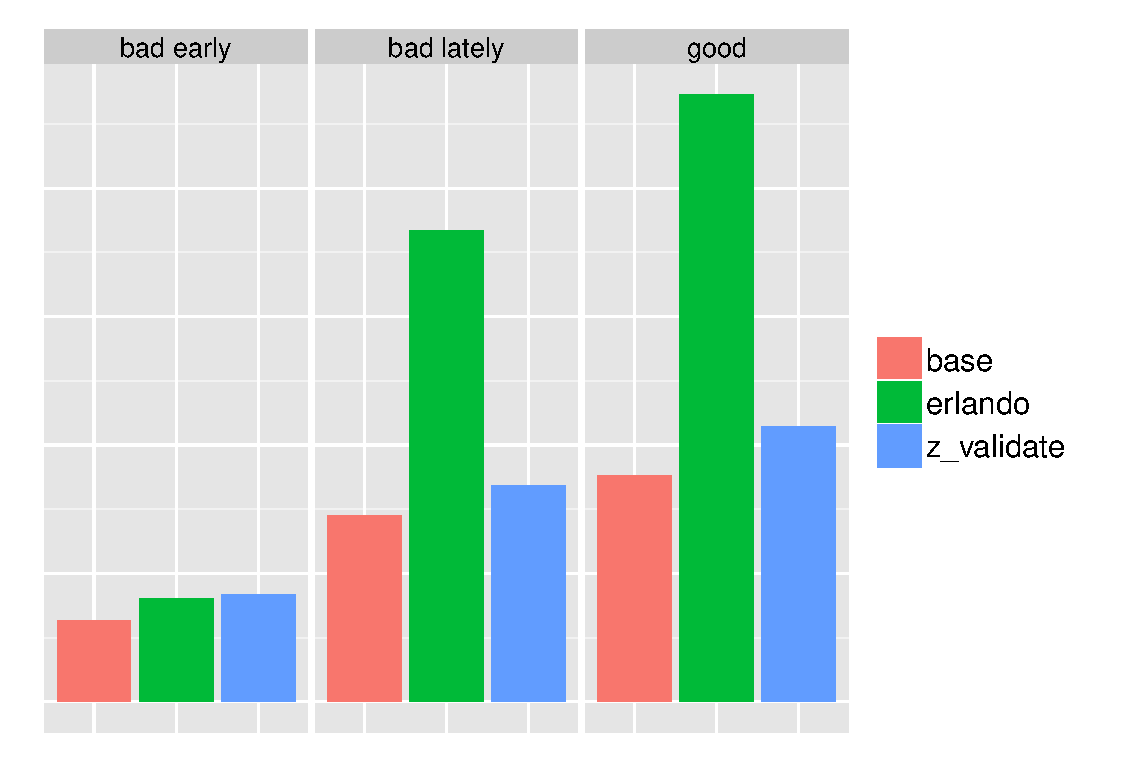
\includegraphics[scale=0.6]{plot.pdf}
  \end{center}
\end{frame}


\begin{frame}{Ошибки}
  \begin{center}
    Все делают ошибки, однако некоторые думают об ошибках так:\vspace{3mm}\\
    \includegraphics[height=6cm]{ostrich}
  \end{center}
\end{frame}

\begin{frame}{Ошибки}
  \begin{center}
    Но лучше делать это так:\vspace{3mm}\\
    \includegraphics[height=6cm]{attack}
  \end{center}
\end{frame}

\begin{frame}{Ошибки}
  \begin{center}
    Для этого нужно знать о враге больше!
  \end{center}
\end{frame}

\begin{frame}{Короткий план доклада}
  \begin{itemize}
  \item общие соображения
    \begin{itemize}
    \item классификация ошибок
    \item о балансе
    \item простые и сложные ошибки
    \item третий путь
    \item всё ещё хуже — ошибки перегрузки, ошибки параллелизма
    \end{itemize}
  \item грязные подробности
    \begin{itemize}
    \item исторически сложившиеся методы обработки ошибок
    \item велосипеды
    \item пример кода
    \end{itemize}
  \end{itemize}
\end{frame}

\begin{frame}{}
  \begin{center}
    \huge Часть 1: общие соображения
  \end{center}
\end{frame}

\begin{frame}{Классификация}
  Наиболее очевидная классификация по времени появления:
  \begin{itemize}
  \item времени компиляции
  \item времени выполнения
  \end{itemize}
\end{frame}

\begin{frame}{Ремарка о балансе}
  Когда ловить ошибки?
  \begin{itemize}
  \item во время компиляции — код либо сложнее, либо многословнее
  \item во время выполнения — падает надёжность, ведь запуск кода не гарантирует его работоспособности
  \end{itemize}
  Необходим баланс между этими крайностями
\end{frame}

\begin{frame}[fragile]{«Простые» ошибки}
  Ошибки бывают очевидными:
  \code{code.py}{1}{3}{python}
  \begin{itemize}
  \item JS: «это не ошибка»
  \item Python: «добавь try/except»
  \item Java: «где типы?»
  \end{itemize}
\end{frame}

\begin{frame}{«Это не ошибка»}
  \begin{center}
    \light{Этот слайд оставлен пустым в память всех жертв плохого дизайна}
  \end{center}
\end{frame}

\begin{frame}{«Добавь try/except»}
  \code{code.py}{5}{10}{python}
  \begin{itemize}
  \item повседневная реальность большинства разработчиков
  \item требует юнит-тестов
  \item 100\% покрытие ничего не гарантирует
  \end{itemize}
\end{frame}

\begin{frame}{«Где типы?»}
  \code{code.java}{1}{7}{java}
  \begin{itemize}
  \item этот код даже не скомпилируется
  \item этого кода слишком много
  \item люди не любят писать много и отказываются от типов вообще
  \end{itemize}
\end{frame}

\begin{frame}{«Где типы?»}
  \code{code.hs}{1}{3}{haskell}
  \begin{itemize}
  \item этот код тоже не скомпилируется
  \item типы a и b однозначно вытекают из соответствующих литералов — зачем их указывать?
  \item компилятор может пытаться выводить типы сам
  \item не все корректные программы могут пройти проверку типов
  \end{itemize}
\end{frame}

\begin{frame}{Проблема статической типизации}
  Ещё раз: \emph{не все корректные программы статически типизируемы}\vspace{2em}\\
  Или: \emph{любая система типов может мешать программисту}
\end{frame}

\begin{frame}{Проблема статической типизации}
  Пример:
  \code{code.java}{17}{23}{java}
\end{frame}
